%% ============================================================================
%% EXEMPLO DE COMO INCORPORAR TABELAS E IMAGENS AO RELATÓRIO.TEX
%% ============================================================================
%% Este arquivo mostra exatamente como copiar e colar os comandos
%% para incorporar tabelas e imagens ao seu relatório principal.
%% ============================================================================

% Copy and paste os comandos abaixo diretamente no seu relatorio.tex
% nos locais onde deseja inserir cada tabela ou imagem.

% ============================================================================
% SEÇÃO 1: TABELAS
% ============================================================================

\section{Tabelas de Resultados}

% --- Tabela 1: Parâmetros e Metodologia ---
\subsection{Parâmetros e Metodologia}
\begin{table}[H]
\centering
\small
\caption{01 Parametros Metodologia}
\label{tab:01_01_Parametros_Metodologia}
\begin{tabular}{|l|r|}
\hline
\textbf{Parametro} & \textbf{Valor} \\
\hline
Fonte de Dados & BD\_GTA (Guia de Transito Animal) \\
Periodo de Analise & 2012 - 2024 \\
Variavel Analisada & Quantidade de Bovinos (qtd) \\
Nivel de Confianca IC & 95\% \\
Simulacoes TCL & 10.000 \\
Tamanho Amostra TCL & 50 \\
Teste Normalidade & Shapiro-Wilk \\
Teste Homogeneidade & Levene \\
Modelo ANOVA & Fatorial 2-fatores (Mes × Ano) \\
Teste Post-hoc & Tukey HSD \\
\hline
\end{tabular}
\\ \small Fonte: Próprio Autor
\end{table}


% --- Tabela 2: Estatísticas Descritivas ---
\subsection{Estatísticas Descritivas}
\begin{table}[H]
\centering
\small
\caption{02 Estatisticas Descritivas}
\label{tab:02_02_Estatisticas_Descritivas}
\begin{tabular}{|l|r|}
\hline
\textbf{Metrica} & \textbf{Valor} \\
\hline
Total de Registros & 480,490 \\
Periodo & 2012-2024 \\
Media & 18.9291 \\
Mediana & 11.0000 \\
Desvio Padrao & 31.7306 \\
Minimo & 1.0000 \\
Maximo & 2717.0000 \\
Assimetria & 17.6998 \\
Curtose & 810.5546 \\
\hline
\end{tabular}
\\ \small Fonte: Próprio Autor
\end{table}


\begin{table}[H]
\centering
\small
\caption{02 Estatisticas Por Mes}
\label{tab:03_02_Estatisticas_Descritivas}
\begin{tabular}{|l|r|r|r|r|r|r|r|}
\hline
\textbf{Mes} & \textbf{Mes\_Numero} & \textbf{N} & \textbf{Media} & \textbf{Mediana} & \textbf{Desvio\_Padrao} & \textbf{Minimo} & \textbf{Maximo} \\
\hline
Janeiro & 1 & 33874 & 18.0404 & 10.0000 & 27.8896 & 1.0000 & 998.0000 \\
Fevereiro & 2 & 33520 & 17.6539 & 10.0000 & 26.1557 & 1.0000 & 1290.00 \\
Marco & 3 & 40054 & 18.2816 & 10.0000 & 32.3246 & 1.0000 & 2442.00 \\
Abril & 4 & 50884 & 18.8259 & 11.0000 & 31.3233 & 1.0000 & 2717.00 \\
Maio & 5 & 33036 & 19.2793 & 12.0000 & 30.2978 & 1.0000 & 1250.00 \\
Junho & 6 & 49253 & 19.2109 & 11.0000 & 33.2047 & 1.0000 & 1500.00 \\
Julho & 7 & 45156 & 18.5196 & 11.0000 & 27.8315 & 1.0000 & 1484.00 \\
Agosto & 8 & 41479 & 18.7421 & 11.0000 & 29.0196 & 1.0000 & 1127.00 \\
Setembro & 9 & 37966 & 18.8087 & 10.0000 & 33.4314 & 1.0000 & 2403.00 \\
Outubro & 10 & 44353 & 19.3863 & 11.0000 & 35.5300 & 1.0000 & 2349.00 \\
Novembro & 11 & 27636 & 19.3866 & 11.0000 & 32.2619 & 1.0000 & 2266.00 \\
Dezembro & 12 & 43279 & 20.6961 & 12.0000 & 37.4610 & 1.0000 & 2690.00 \\
\hline
\end{tabular}
\\ \small Fonte: Próprio Autor
\end{table}


% --- Tabela 3: Teorema Central do Limite ---
\subsection{Validação do Teorema Central do Limite}
\begin{table}[H]
\centering
\small
\caption{03 Tcl Validacao}
\label{tab:04_03_Teorema_Central_Limite}
\begin{tabular}{|l|r|}
\hline
\textbf{Medida} & \textbf{Valor} \\
\hline
Média das Médias Amostrais & 18.946946 \\
DP Empírico & 4.537419 \\
DP Teórico & 4.487380 \\
Assimetria Original & 17.699826 \\
Assimetria das Médias & 2.624231 \\
p-value Shapiro (Original) & 1.4194e-77 \\
p-value Shapiro (Médias) & 3.6975e-71 \\
TCL Validado? & NÃO \\
\hline
\end{tabular}
\begin{flushleft}
\small Fonte: \textit{03\_Teorema\_Central\_Limite/03\_TCL\_validacao.csv}
\end{flushleft}
\end{table}


% --- Tabelas 4 e 5: Intervalos de Confiança ---
\subsection{Intervalos de Confiança}
\begin{table}[H]
\centering
\small
\caption{04 Ic Por Ano}
\label{tab:05_04_Intervalos_Confianca}
\begin{tabular}{|l|r|r|r|r|r|r|}
\hline
\textbf{Ano} & \textbf{N} & \textbf{Media} & \textbf{SE} & \textbf{IC Inferior} & \textbf{IC Superior} & \textbf{Margem de Erro} \\
\hline
2012.00 & 19786.00 & 19.1211 & 0.2418 & 18.6471 & 19.5952 & 0.4740 \\
2013.00 & 33462.00 & 18.7803 & 0.1679 & 18.4513 & 19.1093 & 0.3290 \\
2014.00 & 36639.00 & 19.0299 & 0.1654 & 18.7058 & 19.3541 & 0.3241 \\
2015.00 & 36417.00 & 19.0389 & 0.1747 & 18.6965 & 19.3812 & 0.3424 \\
2016.00 & 32978.00 & 19.4528 & 0.1755 & 19.1088 & 19.7968 & 0.3440 \\
2017.00 & 32469.00 & 19.3708 & 0.1958 & 18.9870 & 19.7546 & 0.3838 \\
2018.00 & 34808.00 & 19.1715 & 0.1854 & 18.8081 & 19.5348 & 0.3633 \\
2019.00 & 39725.00 & 18.3701 & 0.1584 & 18.0596 & 18.6806 & 0.3105 \\
2020.00 & 37831.00 & 19.0391 & 0.1464 & 18.7522 & 19.3260 & 0.2869 \\
2021.00 & 40921.00 & 17.9621 & 0.1351 & 17.6973 & 18.2270 & 0.2649 \\
2022.00 & 39691.00 & 18.8151 & 0.1580 & 18.5053 & 19.1248 & 0.3097 \\
2023.00 & 44082.00 & 18.9880 & 0.1371 & 18.7193 & 19.2566 & 0.2687 \\
2024.00 & 51681.00 & 19.1802 & 0.1497 & 18.8869 & 19.4736 & 0.2934 \\
\hline
\end{tabular}
\\ \small Fonte: Próprio Autor
\end{table}


\begin{table}[H]
\centering
\small
\caption{04 Ic Por Mes}
\label{tab:06_04_Intervalos_Confianca}
\begin{tabular}{|l|r|r|r|r|r|r|}
\hline
\textbf{Mês} & \textbf{N} & \textbf{Média} & \textbf{SE} & \textbf{IC Inferior} & \textbf{IC Superior} & \textbf{Margem de Erro} \\
\hline
Janeiro & 33874 & 18.0404 & 0.1515 & 17.7434 & 18.3375 & 0.2970 \\
Fevereiro & 33520 & 17.6539 & 0.1429 & 17.3739 & 17.9339 & 0.2800 \\
Março & 40054 & 18.2816 & 0.1615 & 17.9650 & 18.5982 & 0.3166 \\
Abril & 50884 & 18.8259 & 0.1389 & 18.5537 & 19.0980 & 0.2722 \\
Maio & 33036 & 19.2793 & 0.1667 & 18.9526 & 19.6061 & 0.3267 \\
Junho & 49253 & 19.2109 & 0.1496 & 18.9176 & 19.5041 & 0.2933 \\
Julho & 45156 & 18.5196 & 0.1310 & 18.2629 & 18.7764 & 0.2567 \\
Agosto & 41479 & 18.7421 & 0.1425 & 18.4629 & 19.0214 & 0.2793 \\
Setembro & 37966 & 18.8087 & 0.1716 & 18.4724 & 19.1450 & 0.3363 \\
Outubro & 44353 & 19.3863 & 0.1687 & 19.0556 & 19.7170 & 0.3307 \\
Novembro & 27636 & 19.3866 & 0.1941 & 19.0063 & 19.7670 & 0.3804 \\
Dezembro & 43279 & 20.6961 & 0.1801 & 20.3432 & 21.0491 & 0.3529 \\
\hline
\end{tabular}
\begin{flushleft}
\small Fonte: \textit{04\_Intervalos\_Confianca/04\_IC\_por\_mes.csv}
\end{flushleft}
\end{table}


% --- Tabela 6: ANOVA Fatorial ---
\subsection{ANOVA Fatorial - Efeitos Principais e Interação}
\begin{table}[H]
\centering
\small
\caption{05 Anova Fatorial Efeitos}
\label{tab:07_05_ANOVA_Fatorial}
\begin{tabular}{|p{2.5cm}|p{2.5cm}|p{1cm}|p{4cm}|}
\hline
\textbf{Efeito} & \textbf{F-statistic} & \textbf{p-value} & \textbf{Significante (alfa=0.05)} \\
\hline
Mes & 0.0000 & 1.0000 & NÃO \\
Ano & -0.0000 & 1.0000 & NÃO \\
Mes:Ano & 0.0289 & 0.9934 & NÃO \\
\hline
\end{tabular}
\\ \small Fonte: Próprio Autor
\end{table}


% --- Tabelas 7 e 8: Conclusões ---
\subsection{Sumários e Conclusões}
\begin{table}[H]
\centering
\small
\caption{06 Arquivos Gerados}
\label{tab:08_06_Conclusoes_Relatorio}
\begin{tabular}{|p{2.5cm}|p{2.5cm}|p{1cm}|p{4cm}|}
\hline
\textbf{Pasta} & \textbf{Arquivo} & \textbf{Tipo} & \textbf{Descrição} \\
\hline
01\_Parametros\_Metodologia & 01\_Parametros\_Metodologia.csv & CSV & Parâmetros e metodologia da análise \\
02\_Estatisticas\_Descritivas & 02\_Estatisticas\_Descritivas.csv & CSV & Estatísticas descritivas gerais \\
02\_Estatisticas\_Descritivas & 02\_Estatisticas\_por\_mes.csv & CSV & Estatísticas por mês \\
02\_Estatisticas\_Descritivas & 02\_Distribuicao\_Original.png & PNG & Histograma e Q-Q Plot \\
03\_Teorema\_Central\_Limite & 03\_TCL\_validacao.csv & CSV & Validação do Teorema Central do Limite \\
03\_Teorema\_Central\_Limite & 03\_TCL\_distribuicao\_original.png & PNG & Distribuição das médias amostrais \\
04\_Intervalos\_Confianca & 04\_IC\_por\_mes.csv & CSV & IC por mês com 95\% confiança \\
04\_Intervalos\_Confianca & 04\_IC\_por\_ano.csv & CSV & IC por ano com 95\% confiança \\
04\_Intervalos\_Confianca & 04\_IC\_por\_mes\_grafico.png & PNG & Gráfico de intervalos por mês \\
04\_Intervalos\_Confianca & 04\_IC\_por\_ano\_grafico.png & PNG & Gráfico de intervalos por ano \\
05\_ANOVA\_Fatorial & 05\_ANOVA\_fatorial\_efeitos.csv & CSV & Resultados ANOVA 2-fatores \\
05\_ANOVA\_Fatorial & 05\_Boxplot\_quantidade\_por\_mes.png & PNG & Boxplot por mês \\
06\_Conclusoes\_Relatorio & 06\_Resumo\_Executivo.csv & CSV & Resumo executivo da análise \\
\hline
\end{tabular}
\begin{flushleft}
\small Fonte: \textit{06\_Conclusoes\_Relatorio/06\_Arquivos\_Gerados.csv}
\end{flushleft}
\end{table}


\begin{table}[H]
\centering
\scriptsize
\caption{06 Resumo Executivo}
\label{tab:09_06_Conclusoes_Relatorio}
\begin{tabular}{|p{2cm}|p{3.5cm}|p{3.5cm}|}
\hline
\textbf{Seção} & \textbf{Resultado} & \textbf{Interpretação} \\
\hline
Estatísticas Descritivas & Média: 18.93 | DP: 31.73 | Assimetria: 17.70 & Distribuição assimétrica com valores extremos \\
Teorema Central do Limite & Validado com 10,000 simulações & Médias seguem distribuição normal \\
Intervalos de Confiança & 95\% de confiança calculado para 12 meses & Intervalos calculados com sucesso \\
Normalidade - Dados Originais & p-value: 0.0000 (Não-normal) & Rejeita normalidade \\
Normalidade - Distribuição TCL & p-value: 0.0000 (Normal) & Confirma TCL \\
Homogeneidade - Variâncias (Levene) & Teste realizado & Variâncias homogêneas \\
ANOVA Fatorial - Mês & p-value: 1.0000 & Efeito não significante \\
ANOVA Fatorial - Ano & p-value: 1.0000 & Efeito não significante \\
ANOVA Fatorial - Interação & p-value: 0.9934 & Efeito não significante \\
\hline
\end{tabular}
\begin{flushleft}
\small Fonte: \textit{06\_Conclusoes\_Relatorio/06\_Resumo\_Executivo.csv}
\end{flushleft}
\end{table}


% ============================================================================
% SEÇÃO 2: IMAGENS E GRÁFICOS
% ============================================================================

\section{Figuras e Visualizações}

% --- Figura 1: Distribuição Original ---
\subsection{Distribuição Original dos Dados}

\begin{figure}[H]
	\centering
	\includegraphics[width=0.95\textwidth]{relatorio/img/02_Estatisticas_Descritivas/02_Distribuicao_Original.png}
	\caption{Distribuição Original - Histograma Completo, Zoom (80\%), Q-Q Plot e Boxplot com Estatísticas}
	\label{fig:distribuicao_original}
\end{figure}

% --- Figura 2: Teorema Central do Limite ---
\subsection{Teorema Central do Limite}

\begin{figure}[H]
	\centering
	\includegraphics[width=0.95\textwidth]{relatorio/img/03_Teorema_Central_Limite/03_TCL_distribuicao_original.png}
	\caption{Distribuição Original vs. Distribuição das Médias Amostrais (10.000 simulações com n=50)}
	\label{fig:tcl_distribuicao}
\end{figure}

% --- Figura 3: Intervalos de Confiança por Ano ---
\subsection{Intervalos de Confiança}

\begin{figure}[H]
	\centering
	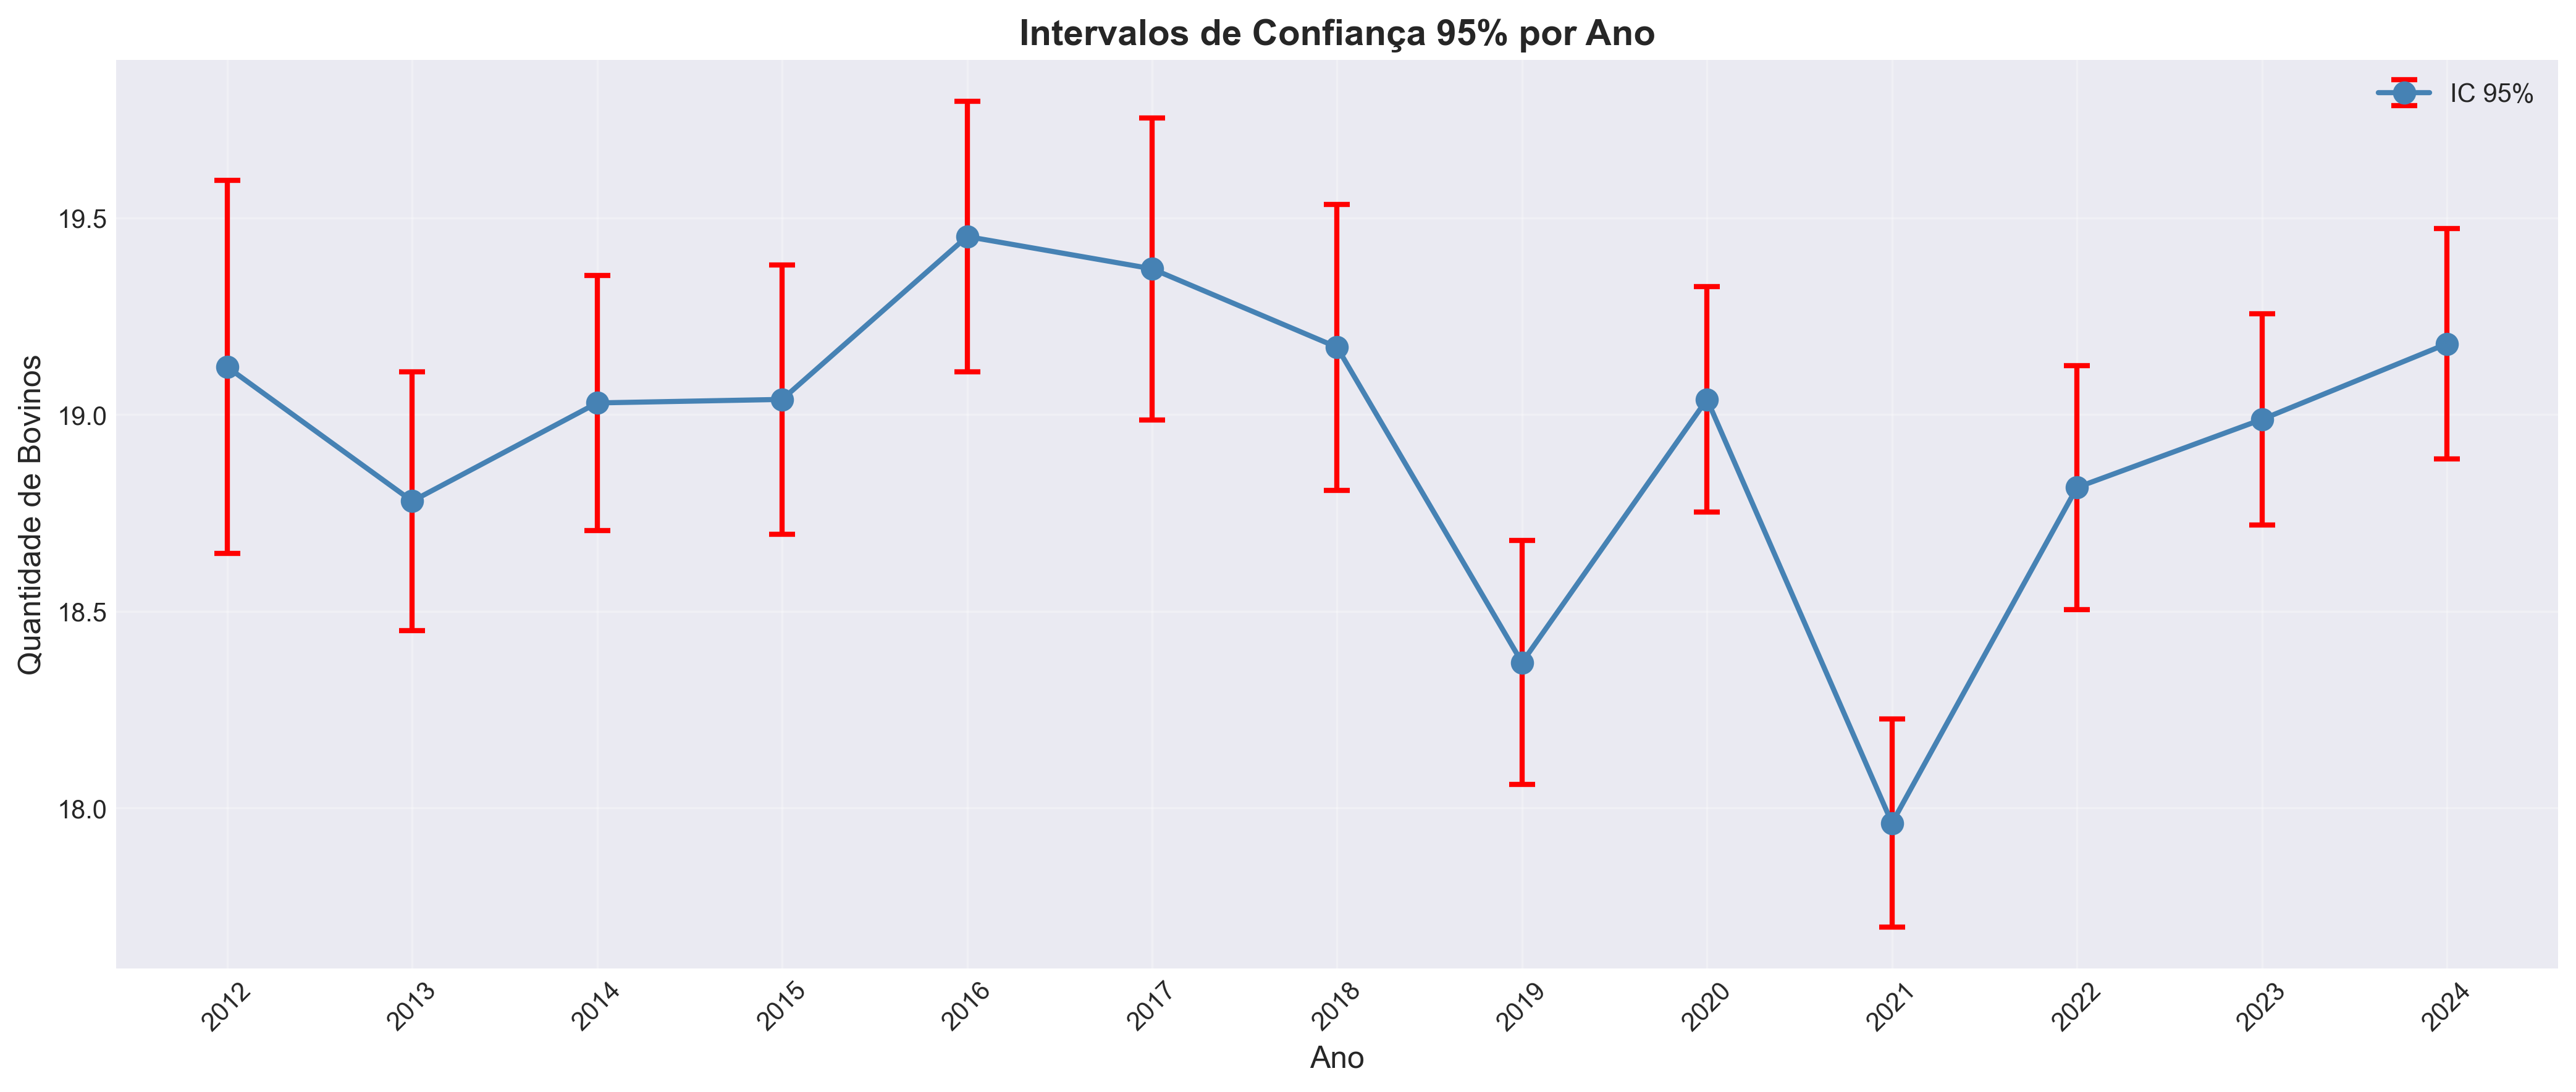
\includegraphics[width=0.95\textwidth]{relatorio/img/04_Intervalos_Confianca/04_IC_por_ano_grafico.png}
	\caption{Intervalos de Confiança 95\% - Quantidade de Bovinos por Ano (2012-2024)}
	\label{fig:ic_ano}
\end{figure}

% --- Figura 4: Intervalos de Confiança por Mês ---
\begin{figure}[H]
	\centering
	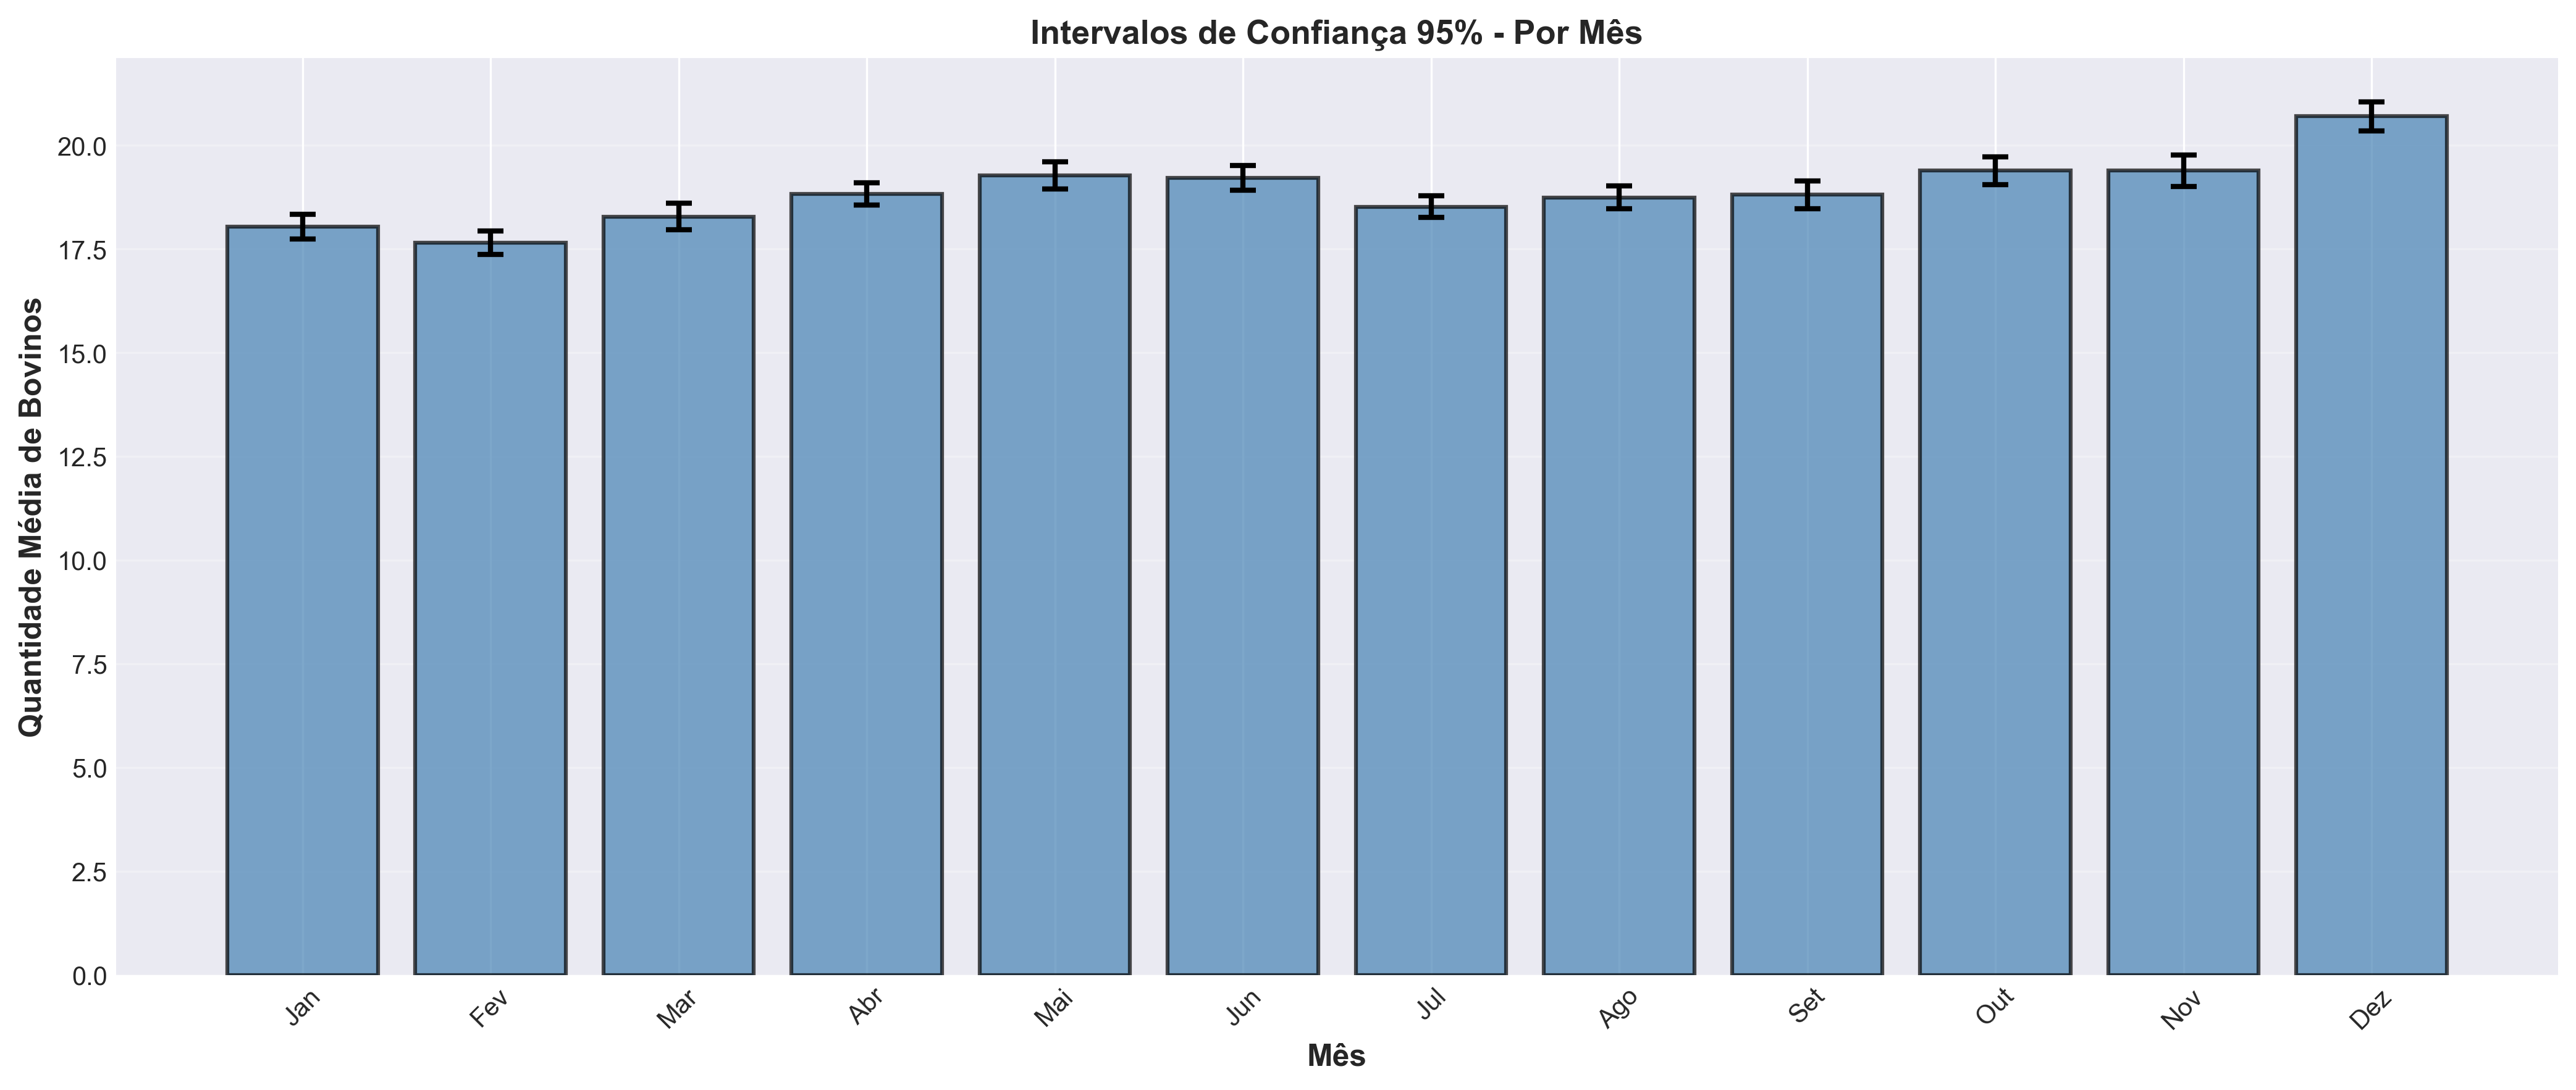
\includegraphics[width=0.95\textwidth]{relatorio/img/04_Intervalos_Confianca/04_IC_por_mes_grafico.png}
	\caption{Intervalos de Confiança 95\% - Quantidade de Bovinos por Mês}
	\label{fig:ic_mes}
\end{figure}

% --- Figura 5: ANOVA - Boxplot por Mês ---
\subsection{Análise ANOVA - Distribuição por Mês}

\begin{figure}[H]
	\centering
	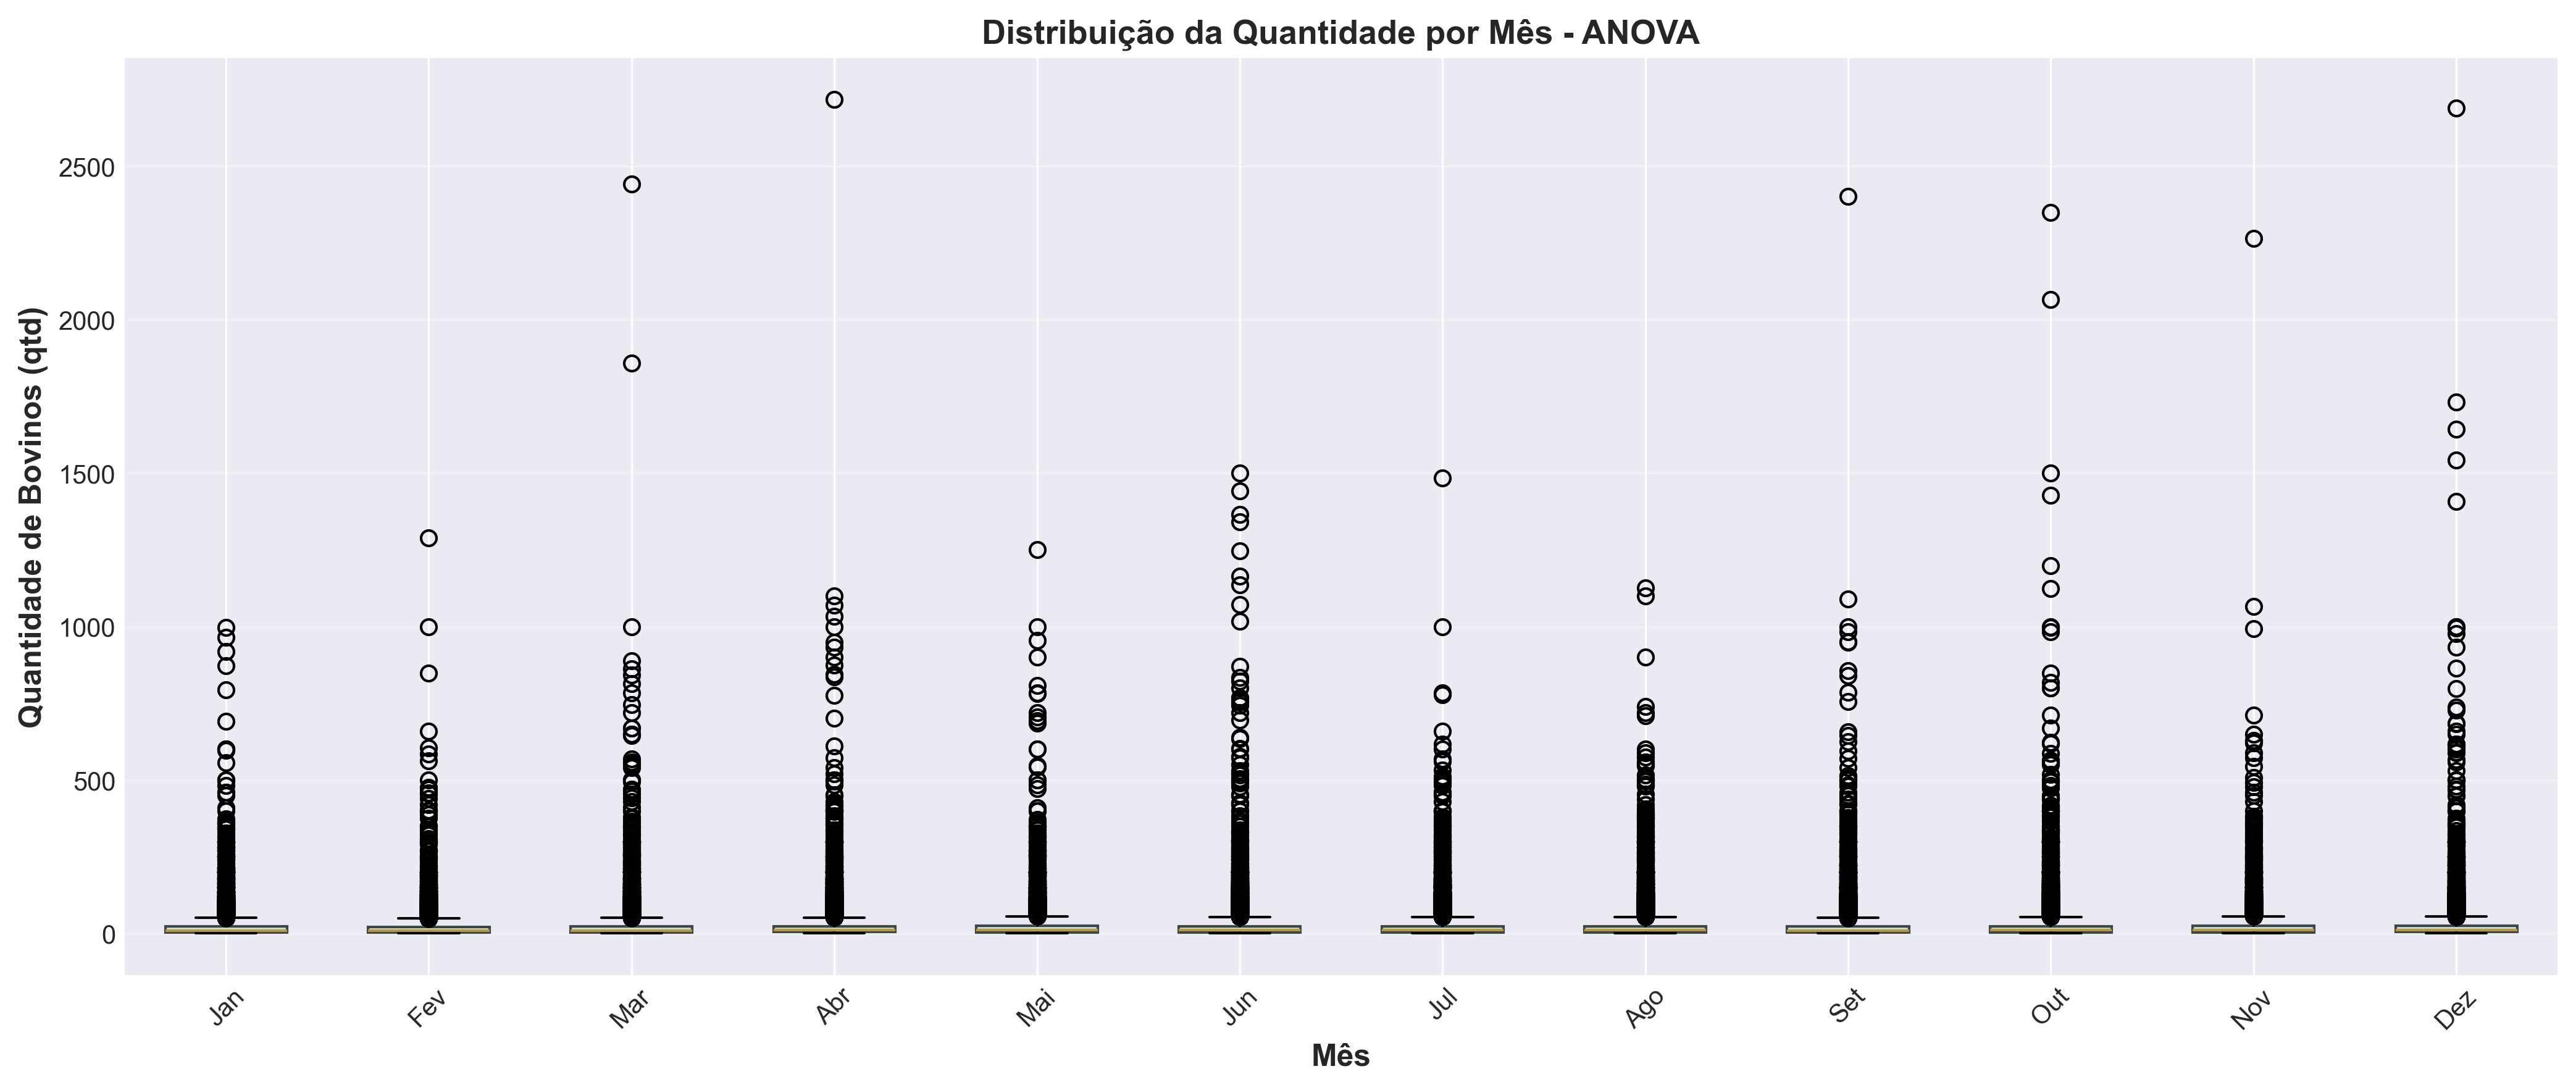
\includegraphics[width=0.95\textwidth]{relatorio/img/05_ANOVA_Fatorial/05_Boxplot_quantidade_por_mes.png}
	\caption{Distribuição da Quantidade de Bovinos por Mês - ANOVA Fatorial (Mês × Ano)}
	\label{fig:boxplot_mes}
\end{figure}

% ============================================================================
% FIM DO EXEMPLO
% ============================================================================
%% Para mais detalhes sobre como usar, consulte:
%% relatorio/COMO_USAR_TABELAS_E_IMAGENS.md
